\input{preambula.inc}
\tikzstyle{every node}=[rectangle, draw=none, font=\Large, text=cLines, inner sep=1pt, minimum size=5mm]
\begin{tikzpicture}
  \node (a) {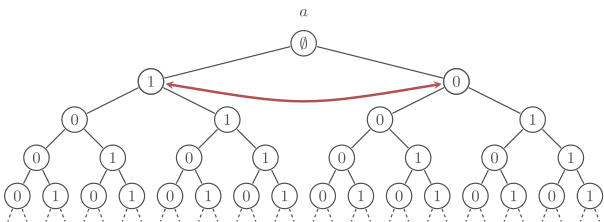
\includegraphics[scale=0.5]{AutomorphismA}};
  \path (a) ++(0,-2.5) node (caption) {Automorphism $a$};
  \path (a) ++(11,0) node (b)
        {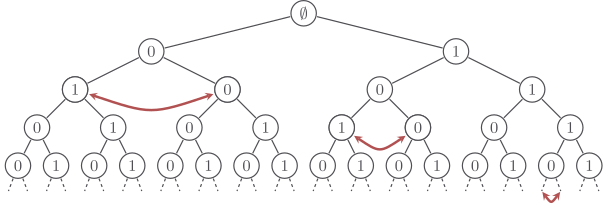
\includegraphics[scale=0.5]{AutomorphismB}};
  \path (b) ++(0,-2.5) node (captionb) {Automorphism $b$};
  \path (caption) ++(0,-3) node (c)
        {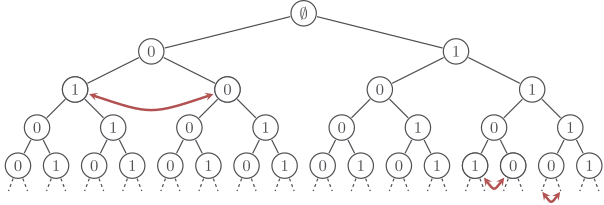
\includegraphics[scale=0.5]{AutomorphismC}};
  \path (c) ++(0,-2.5) node (caption) {Automorphism $c$};
  \path (captionb) ++(0,-3) node (d)
        {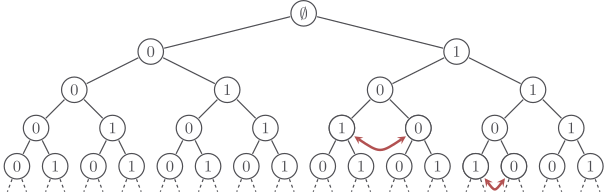
\includegraphics[scale=0.5]{AutomorphismD}};
  \path (d) ++(0,-2.5) node {Automorphism $d$};
\end{tikzpicture}

\end{document}
